\documentclass[12pt]{article}

% Solutions toggle
\newif\ifsolutions
\solutionsfalse
%% \solutionstrue

% ASSIGNMENT NUMBER
\newcommand{\hwnumber}{5}
\newcommand{\booksection}{}
\newcommand{\duedate}{}
% -------------

%%% Packages
\usepackage[margin=1in, footskip=24pt, headheight=24pt]{geometry}
\usepackage{amsmath, amssymb, amsthm, graphicx}
\usepackage{mathtools}
\DeclarePairedDelimiter\ceil{\lceil}{\rceil}
\DeclarePairedDelimiter\floor{\lfloor}{\rfloor}
\usepackage[colorlinks, urlcolor=blue]{hyperref}
\usepackage{color}
\usepackage{comment}
\usepackage{enumerate}
\usepackage{lastpage}
\usepackage{multirow, multicol}
\usepackage{tikz}
\usetikzlibrary{matrix,decorations.text,decorations.pathmorphing,decorations.markings,arrows,calc,shapes.geometric,patterns,shadows,intersections,decorations.markings,decorations.pathreplacing,decorations.pathreplacing,backgrounds,angles,quotes}
\usepackage{pgfplots}
\pgfplotsset{compat=1.16}

\usepackage{fancyhdr}

\pagestyle{fancy}
%% \renewcommand{\familydefault}{\sfdefault}

\newcommand{\R}{\mathbb{R}}
\newcommand{\ddx}{\frac{d}{dx}}

\global\long\def\V#1{\boldsymbol{#1}} %vector
\global\long\def\M#1{\boldsymbol{#1}} %matrix

\global\long\def\D#1{\Delta#1} %\D{t} for time step size
\global\long\def\d#1{\delta#1} %\d{t} for small increment

\global\long\def\norm#1{\left\Vert #1\right\Vert }
\global\long\def\abs#1{\left|#1\right|}

\global\long\def\grad{\M{\nabla}}
\global\long\def\av#1{\left\langle #1\right\rangle }

% HEADER MACROS
\newcommand{\term}{Spring 2022 \& 2023}
\newcommand{\coursename}{Intro Math Modeling}
\newcommand{\coursenumber}{MATH-UA 251}
\newcommand{\course}{\coursename \ (\coursenumber)}

\fancyhead[RO]{\term}
\fancyhead[LO]{\course}
% -------------

%%% Theorem Styles
\theoremstyle{definition}
\newtheorem{ex}{Exercise}

%%%%%%%%%%%%%%%%%%%%%%%% Solutions %%%%%%%%%%%%%%%%%%%%%%%%%%%%%
% \begin{solution} and \begin{answerspace} must be at the beginning of the line.
% Doesn't work inside the \myversions command. Use if statements instead.
% No underscores in comment names

\ifsolutions
\newenvironment{solution}{\color{blue}}{} \excludecomment{answerspace} \newenvironment{notes}{\color{red} \noindent Grading Notes:}{}
\else
\excludecomment{notes} \excludecomment{solution} \includecomment{answerspace} 
\fi
%%%%%%%%%%%%%%%%%%%% End Solutions %%%%%%%%%%%%%%%%%%%%%%%e}


\begin{document}
% HEADER
\begin{center}
%% \ifsolutions
%%   \textbf{\Large Homework \hwnumber\ - \booksection\ (Solutions)}\\
%% \else
%%   \textbf{\Large Homework \hwnumber\ - \booksection}\\
%% \fi
\ifsolutions
  \textbf{\Large Homework \hwnumber\ (Solutions)}\\
\else
  \textbf{\Large Homework \hwnumber}\\
\fi
\vspace{12pt}
Due date: someday, sometime! \duedate

Submit on NYU Brightspace.
\end{center}

%% \noindent Please give complete, well-written solutions to the following exercise. Provide sufficient justification and explanation for a classmate who has not worked on the exercise to understand your solution.


\begin{ex}
  
  [100 pts] Consider the following population growth models:
  \begin{enumerate}[(i)]\setlength{\itemsep}{0pt}
  \item $\displaystyle{\frac{\dot{N}}{N}=-a\ln(bN)}$\\
    with $a,b$ as positive constants. Interpret the constants $a$ and $b$ biologically. (You might find it helpful to analyze their dimensions.)
  \item $\displaystyle{\frac{\dot{N}}{N}=r-a(N-b)^2}$\\
    with $r,a,b$ as positive constants. Find a relation between these constants, so that the per capita growth rate $\dot{N}/N\to 0$ as $N\to 0$.
  \end{enumerate}
  For each of the above models,
  \begin{itemize}\setlength{\itemsep}{0pt}
      \item Analytically find the fixed points $N^*$ by letting $\dot{N}=0$. Hint: sometimes, $\dot{N}$ is not defined at a fixed point (in particular unstable fixed points); under such circumstances, look for $N^*$ for which $\lim_{N\to N^*}\dot{N}=0$.
      \item Use linear stability analysis to identify the stability of the fixed points. If not possible, find the stability by a graphical analysis from the next steps.
      \item Sketch (by hand) $\dot{N}$ versus $N$, show the fixed points on the graph, along with the flow field. (Do \textbf{NOT} use computer to make this plot! Instead, use your understanding from calculus and make a qualitative plot.)
      \item Sketch (by hand) $N(t)$ versus time for various initial values $N_0$. (Again, do \textbf{NOT} use computer.)
  \end{itemize}

\noindent\textbf{\textcolor{red}{notes:} }Solutions without details of the work and interpretation of the results will not receive full credits. Your sketches should show the important qualitative features of each growth model (e.g., concavities, approach to fixed points). They should also clearly demonstrate the differences, if any, between the two models.

\begin{solution}
  \begin{enumerate}[(i)]\setlength{\itemsep}{0pt}
  \item The dimensions of $a$ are $\{\mathrm{numbers}/\mathrm{time}\}$, and hence, $a$ corresponds to the growth rate scale. $b$ is dimensionless $\{1/\mathrm{numbers}\}$, and $1/b$ is the carrying capacity. See below for more details.

    \begin{itemize}\setlength{\itemsep}{0pt}
    \item Let $\dot{N}=-aN\ln(bN)=0$; clearly, $N^*=1/b$ is a fixed point. Furthermore, note that
    $$\lim_{N\to 0}(-aN\ln(bN))=0,$$
      and, therefore, $N^*=0$ is the other fixed point of the system.
    \item We evaluate $f'(N)$ where $f(N)=-aN\ln(bN)$:
      $$f'(N)=-a\ln(bN)-a.$$
      We note that $\lim_{N^*\to0}f'(N^*)\to\infty$ ($N^*=0$ is unstable), and $f'(1/b)=-a$ ($N^*=1/b$ is stable).
    \item $\dot{N}$ versus $N$

    \begin{center}
    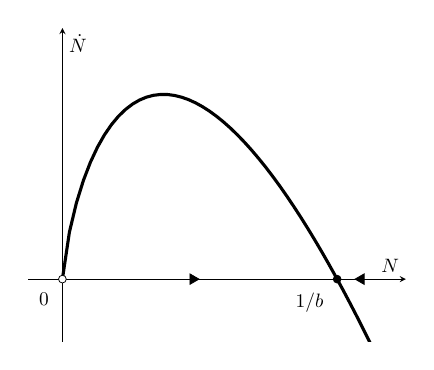
\begin{tikzpicture}[scale=0.7]
    \begin{axis}[xmin=-0.5,xmax=5,ymin=-0.5,ymax=2,
    axis lines=middle,
    xtick={0},
    ytick={0},
    xlabel={$N$},
    ylabel={$\dot{N}$},
    samples=50
      ]
      \coordinate (O) at (0,0);
      \coordinate (K) at (4,0);
      \node[anchor=north east] at ($(O)+(-135:5pt)$) {$0$};
      \node[anchor=north east] at ($(K)+(-135:5pt)$) {$1/b$};
      \addplot[domain=0:5,ultra thick] (x,{-x*ln(x/4)});
      \addplot[mark=*,fill=white] coordinates {(0,0)};
      \addplot[mark=*] coordinates {(4,0)};
      \addplot[->,>=triangle 60] coordinates {(1.75,0) (2,0)};
      \addplot[->,>=triangle 60] coordinates {(4.5,0) (4.25,0)};
      
    \end{axis}
    \end{tikzpicture}
    \end{center}

    \item $N(t)$ versus $t$ for different $N_0$
    \begin{figure}[h]
      \centering
      \resizebox{0.6\textwidth}{!}{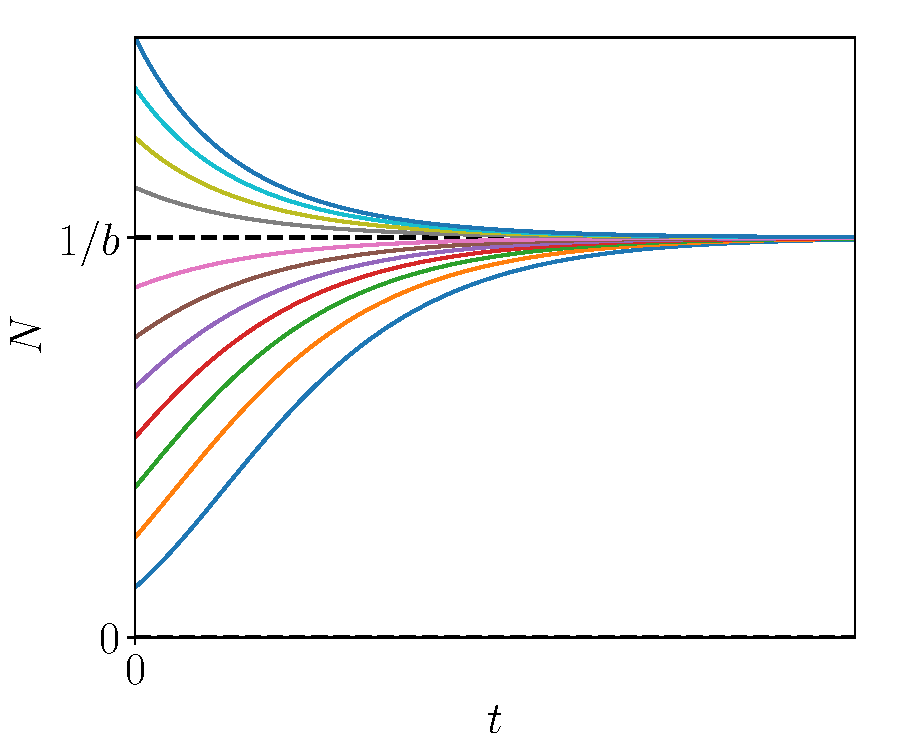
\includegraphics{popGrowth_i.pdf}}
    \end{figure}

    \end{itemize}

  \item We need $\dot{N}/N=r-a(N-b)^2$ to be zero at $N=0$:
    $$0=r-ab^2\Rightarrow b=\sqrt{r/a}.$$

    \begin{itemize}\setlength{\itemsep}{0pt}
    \item Let $\dot{N}=N\left[r-a(N-b)^2\right]=0$; $N^*=0$ is clearly a fixed point. Equating the expression in the brackets to zero yields
      $$r-a(N-b)^2=0\Rightarrow N^*=b\pm\sqrt{\frac{r}{a}}.$$
      Note that the minus sign gives $N^*=0$ since $b=\sqrt{r/a}$. Therefore, we have two fixed points $N^*=0$ and $N^*=2b$.
    \item For $f(N)=N\left[r-a(N-b)^2\right]$,
      $$f'(N)=r-a(N-b)^2-2aN(N-b)$$
      We note that
      $$f'(2b)=r-a(2b-b)^2-2a\cdot(2b)(2b-b)=r-ab^2-4ab^2=-4ab^2<0,$$
      and so, $N^*=2b$ is stable. However, at $N^*=0$,
      $$f'(0)=r-a(0-b)^2-0=r-ab^2=0.$$
      Therefore, linear stability analysis does not provide any information as to whether $N^*=0$ is stable or unstable.
      
    \item $\dot{N}$ versus $N$

    \begin{center}
    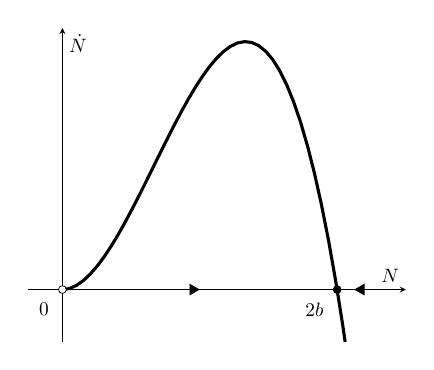
\begin{tikzpicture}[scale=0.7]
    \begin{axis}[xmin=-0.5,xmax=5,ymin=-2,ymax=10,
    axis lines=middle,
    xtick={0},
    ytick={0},
    xlabel={$N$},
    ylabel={$\dot{N}$},
    samples=50
      ]
      \coordinate (O) at (0,0);
      \coordinate (K) at (4,0);
      \node[anchor=north east] at ($(O)+(-135:5pt)$) {$0$};
      \node[anchor=north east] at ($(K)+(-135:5pt)$) {$2b$};
      \addplot[domain=0:5,ultra thick] (x,{x*(4-1*pow(x-2,2))});
      \addplot[mark=*,fill=white] coordinates {(0,0)};
      \addplot[mark=*] coordinates {(4,0)};
      \addplot[->,>=triangle 60] coordinates {(1.75,0) (2,0)};
      \addplot[->,>=triangle 60] coordinates {(4.5,0) (4.25,0)};
      
    \end{axis}
    \end{tikzpicture}
    \end{center}

    From this figure, it is evident that $N^*=0$ is unstable.
    
    \item $N(t)$ versus $t$ for different $N_0$
    \begin{figure}[h]
      \centering
      \resizebox{0.6\textwidth}{!}{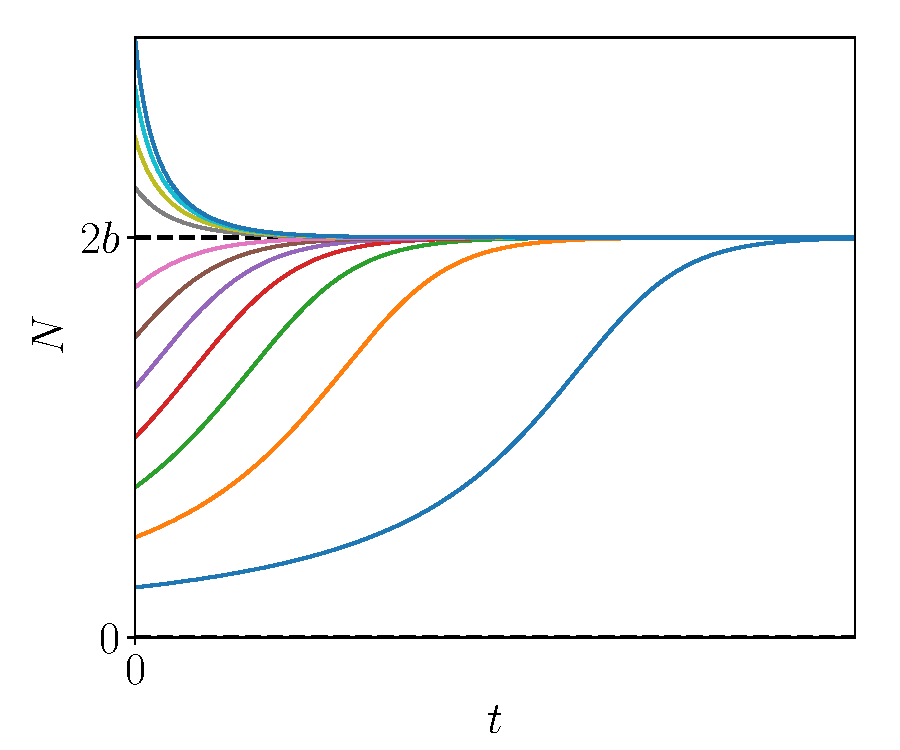
\includegraphics{popGrowth_ii.pdf}}
    \end{figure}
    
    A key feature here, is that, compared to case (i), it takes much longer for a small population to start growing fast. Note that we can find the inflection point by
    \begin{align*}
      \frac{df}{dN}=&r-a(N-b)^2-2aN(N-b)=0\\
      \Rightarrow &\frac{r}{a}-(N-b)^2-2N(N-b)=b^2-(N-b)^2-2N(N-b)=N(-3N+4b)=0\\
      \Rightarrow &N=0,\quad N=\tfrac{4}{3}b.
    \end{align*}
    \end{itemize}
    
  \end{enumerate}
  
\end{solution}
\end{ex}


\end{document}
